
Una vez elegido nuestro modelo debemos de comprobar que efectivamente cumple las condiciones bajo las cuales están sustentadas:

\begin{itemize}
    \item Parametros significativos 
    \item Independecia de los residuos
    \item Independecia de los residuos al cuadrado 
    \item La distribucion empirica se distribuye con una t-student sesgada  

\end{itemize}

\bigskip
\subsection{Parametros Significativos}
\bigskip
En la tabla \ref{Caracteristicas del modelo} se muestran los valores estimados de los parámetros, las respectivas desviaciones estándar, y el p-valor correspondiente a las pruebas de hipótesis son 
\bigskip
$$H_0:\theta_i =0 \quad vs.\quad H_1:\theta_i \not= 0$$

\newpage

   Para estos parámetros. La hipótesis $H_{0}$ se rechaza a un nivel de significancia del 5$\%$
   

\begin{table}[htbp]

\begin{center}
    

\begin{tabular}[!h]{|c | c | c | } \hline
	
	\rowcolor{cyan} \multicolumn{3}{ |c| }{ \textbf{Modelo GARCH (1,2)   }} \\ \hline
	 \hline
	

\rowcolor{red}  Parámetro & Valor Estimado & P-value\\\hline
	  
  $\mu$      &	0.001827	& 	0.000024  \\\hline
  $ar_1$     &	-0.985978   & 0.000000   \\\hline
  $ma_1$     &	0.989861    & 	0.000000 \\\hline
  $\omega$   &	0.000018    & 	0.000131 \\\hline
  $\alpha_1$ &	0.053250 	&	0.000000 \\\hline
  $\beta_1$  &	0.120970	&	0.004485 \\\hline
  $\beta_2$  &	0.816019	&	0.000000 \\\hline
    skew     & 1.073804 	&	0.000000 \\\hline
    shape     &	3.153194	&	0.000000 \\\hline
    	     
	
	\end{tabular}

	\label{Caracteristicas del modelo}
	\caption{Caracteristicas del modelo}
\end{center}

\end{table}
 
 Resumiendo, de esta tabla podemos decir que tenemos suficiente información estadística para decir que todos  los parámetros son significativamente distintos de 0. La ecuación de varianza de este modelo resulta ser:
 
 \begin{equation}
   \sigma_t^2 =0.000018+  0.053250  \epsilon_{t-1}^2 + 0.120970  \sigma_{t-1}^2 + 0.120970  \sigma_{t-2}^2
\end{equation}

Y el modelo de los rendimientos es:

 \begin{equation}
   r_t =  0.001827 - 0.985978(r_{t-1} - 0.001827) + 0.989861\epsilon_{t-1} +  \epsilon_t
\end{equation}



 \subsection{Independencia de residuos}
 Para este supuesto se realizó la prueba de hipótesis Ljung-Box cuyas hipótesis son 
 
 \begin{itemize}
  \centering
    \item[$H_{0}$] \textit{: Los residuales se distribuyen de forma independiente } 
    \item [$H_{1}$] \textit{:Los residuales no se distribuyen de forma independiente }
 \end{itemize}
 \bigskip
los resultados de esta prueba se pueden apreciar en la tabla \ref{Ljung-Box Test en Residuos estandarizados}.
\bigskip

\begin{table}[h]
 
\begin{center}
    

\begin{tabular}[!h]{ |c |  c |  } \hline
	
	\rowcolor{cyan} \multicolumn{2}{ |c| }{ \textbf{Ljung-Box Test en Residuos estandarizados }} \\ \hline
	 \hline
	

\rowcolor{red}   Lag & P-value \\\hline
	  
	                1	& 0.07379 \\\hline
                    5	& 0.18209  \\\hline
                    9	& 0.57767   \\\hline
                    
	
	\end{tabular}
      \caption{Ljung-Box Test en Residuos estandarizados}
	\label{Ljung-Box Test en Residuos estandarizados}
	
\end{center}

\end{table}



Como conclusión de esta tabla podemos decir que los residuos estandarizados obtenidos por el modelo no tienen correlación entre sí para los retrasos  1, 5 y 9. 
\\
\newpage
 
Esto se puede apreciar visualmente en la gráfica \ref{ACF Residuales} en la cual se muestra un buen comportamiento de las autocorrelaciones de los residuos estandarizados pues la mayoría de ellas se encuentran comprendidas en las bandas de confianza.


\begin{figure}[h]
    \centering
    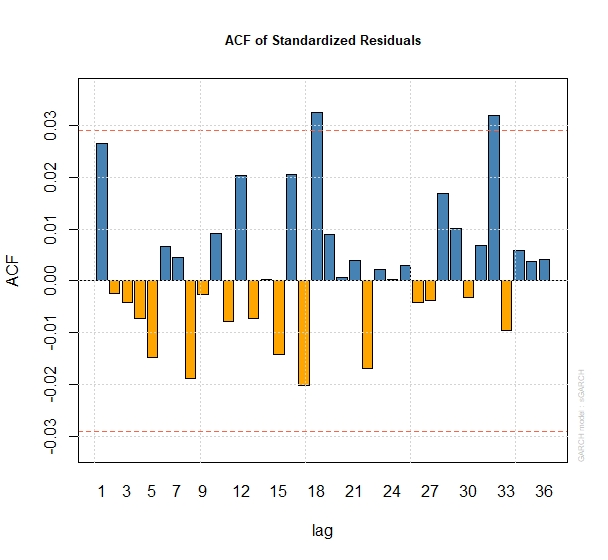
\includegraphics[scale=.4]{Graficos/ACF Residuales sta.jpeg}
    \caption{ACF Residuales}
    \label{ACF Residuales}
\end{figure}

\bigskip
Ahora como se menciono en la implementación del modelo, los modelos \textbf{GARCH}  dependen del cuadrado de los errores retrasados p periodos atrás
es por ello que es importante aplicar la misma prueba de hipótesis a los residuos cuadráticos estandarizados.
\\
Los resultados de esta prueba se pueden ver en la tabla \ref{Ljung-Box Test en Residuos cuadraticos estandarizados}.


\begin{table}[!h]
 
\begin{center}
    

\begin{tabular}[!h]{ |c |  c |  } \hline
	
	\rowcolor{cyan} \multicolumn{2}{ |c| }{ \textbf{Ljung-Box Test en Residuos cuadráticos estandarizados }} \\ \hline
	 \hline
	

\rowcolor{red}   Lag & P-value \\\hline
	  
	                1	& 0.9838 \\\hline
                    8	& 0.9914  \\\hline
                    14	& 0.9980  \\\hline
                    
	
	\end{tabular}

\caption{Ljung-Box Test en Residuos cuadraticos estandarizados}
	\label{Ljung-Box Test en Residuos cuadraticos estandarizados}
	
\end{center}

\end{table}



De esta manera, podemos afirmar que tenemos suficiente información estadística para decir que los residuales cuadráticos estandarizados son independientes, siendo esto confirmado  por la gráfica \ref{ACF cuadraticos}.
\bigskip


\begin{figure}[h]
    \centering
    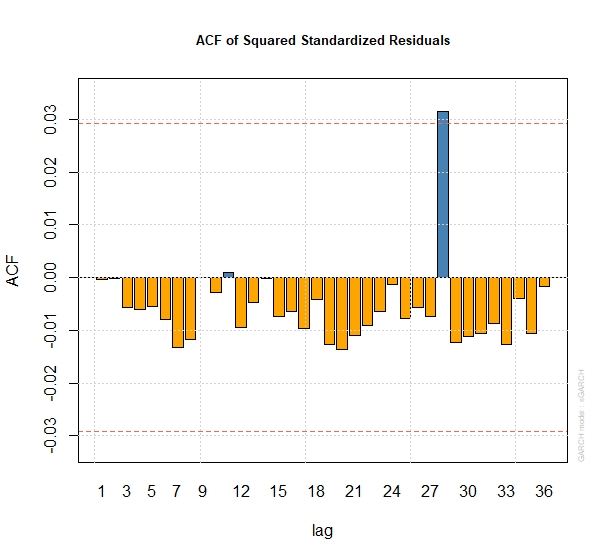
\includegraphics[scale=.5]{Graficos/ACF Residuales.jpeg}
     \caption{ACF Residuales cuadraticos}
    \label{ACF cuadraticos}
\end{figure}




\subsection{Ajuste a ditribucion Empirica}
\bigskip
Para determinar si la distribución propuesta es correcta, en este caso la t-student sesgada, se llevo a cabo una prueba de bondad ajuste, la cual  compara la distribución teórica de los residuos estandarizados con la distribución empírica seleccionada. La hipótesis nula es que la distribución empírica y teórica es idéntica.
\bigskip
\begin{table}[h]

\begin{center}
    

\begin{tabular}[!h]{|c | c | } \hline
	
	\rowcolor{cyan} \multicolumn{2}{ |c| }{ \textbf{Prueba de Bondad de Ajuste de Pearson}} \\ \hline
	 \hline
	

\rowcolor{red}  Group  & P-value\\\hline
	  
  20   	& 	0.1806 \\\hline
  30    &   0.1972 \\\hline
  40    & 	0.1954 \\\hline
  50    & 	0.1024 \\\hline

	
	\end{tabular}

	\label{Person}
	\caption{Prueba de Hipotesis Person}
	
\end{center}

\end{table}


 Notemos que en cualquier caso el p-value$>$ 0.05 por lo que no se rechaza la hipotesis nula, para comprobar esto, podemos observar el qq-plot y el histograma de los residuos.
 
 \begin{figure}[h]
    \centering
    \subfigure{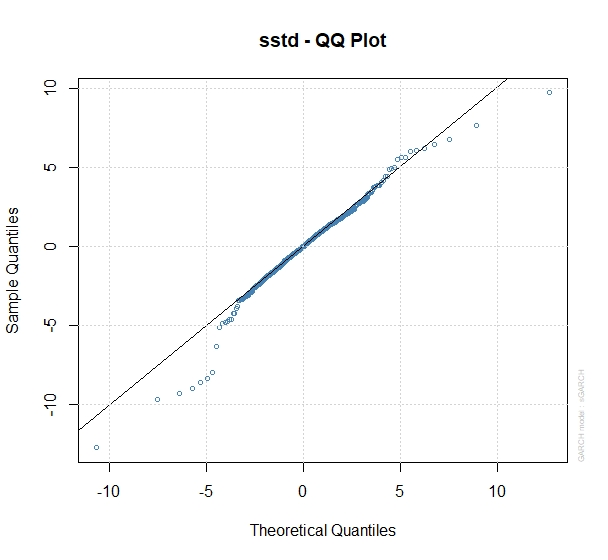
\includegraphics[width=60mm]{Graficos/QQPlotSST.jpeg}}\vspace{10mm}
    \subfigure{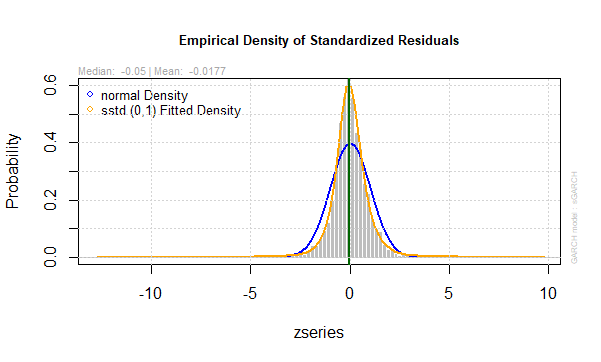
\includegraphics[width=100mm]{Graficos/DensityResiduals.png}}
    \caption{Ajuste a distribucion de t-studet.} 
    \label{Ajuste a distribucion de t-studet.}
\end{figure}
 
 
 
\subsection{Media cero de los residuos}
\bigskip
 Para verificar el supuesto de que los residuos mantienen una media igual a 0 se efectuó la prueba t-Student cuyo p-value nos permite afirmar este hecho. En este caso el p-value resulto de 0.3355 por lo que no se rechaza la hipótesis nula.
 

 Además de ello si hacemos el calculo de la media de los residuo veremos que esta resulta -0.0005258295, un valor muy cercano al 0.
 \newpage
\subsection{Varianza constante de los residuos}

 La  manera  de  comprobar  dicho  supuesto  sobre  el  ruido  blanco  del  modelo  es  mediante  herramientas gráficas.
 
\begin{figure}[!h]
    \centering
    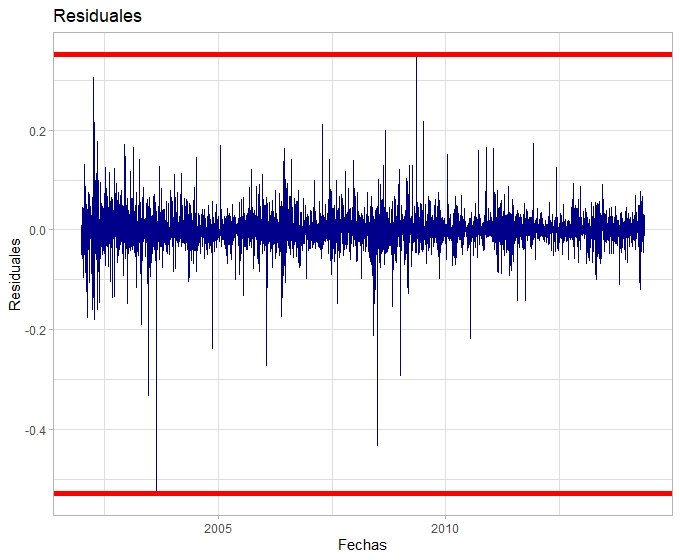
\includegraphics[width=0.55\textwidth]{Graficos/ResidualesApa.jpeg}
      \caption{Residuales}
    \label{Graficas de residuos}
\end{figure}
\bigskip

 
 Como  es  posible  observar,  la  varianza  de  los  residuales  no  es  creciente  pues  se  pueden  encerrar las observaciones entre dos bandas. En nuestro caso las bandas corresponden al valor mínimo y máximo delos residuos, por lo tanto, con total seguridad podemos decir que el supuesto se cumple con  éxito.
 
